\documentclass{article}

\usepackage[utf8]{inputenc}
\usepackage[brazil]{babel}

\title{Exercício 8: Seleção de Características}
\author{Rúbia Reis Guerra \\ 2013031143}

\usepackage{Sweave}
\begin{document}
\Sconcordance{concordance:selecao.tex:selecao.Rnw:%
1 8 1 1 0 7 1 1 2 1 0 4 1 1 9 11 0 1 2 1 1 1 4 3 0 3 1 1 2 1 1 1 2 2 1 %
4 0 1 2 1 4 3 0 1 1 7 0 1 2 1 4 3 0 1 5 4 0 1 1 55 0 1 3 2 1 1 4 3 0 1 %
1 4 0 1 2 1 1 1 3 2 0 2 1 4 0 1 2 1 1 1 3 2 0 2 1 4 0 1 2 1 3 2 0 2 1 4 %
0 1 2 1 3 2 0 2 1 4 0 1 2 1 3 2 0 2 1 4 0 1 2 1 3 2 0 2 1 4 0 1 2 1 3 2 %
0 2 1 4 0 1 2 1 1 1 3 2 0 2 1 4 0 1 2 1 3 2 0 2 1 4 0 1 2 1 1 1 3 2 0 2 %
1 4 0 1 2 1 1 1 3 2 0 2 1 4 0 1 2 1 1}


\maketitle

\section{Seleção de Características}
Nesta atividade, foi proposta a análise do dataset \textit{BCW (BreastCancer)}, implementando a seleção de características via Kmeans, F-Score e clustering hieráquico.

\begin{Schunk}
\begin{Sinput}
> rm(list=ls())
> library('MASS')
> library('mlbench')
> library('mclust')
> library('stats')
> fscore <- function(X,c1,c2,n){
+   f <- c()
+   for(i in 1:n)
+   {
+     f[i] <- ((mean(c1[,i]) - mean(X[,i]))^2
+              +(mean(c2[,i]) - mean(X[,i]))^2)/(sd(c1[,i])^2+sd(c2[,i])^2)
+   }
+   return(f)
+ }
\end{Sinput}
\end{Schunk}


\begin{Schunk}
\begin{Sinput}
> ###########################
> # Dataset BreastCancer #
> data(BreastCancer)
> X<- data.matrix(BreastCancer[,2:10])
> X[is.na(X)] <- 0
> Y <- as.numeric(BreastCancer$Class)
> c1 <- X[which(Y==1),]
> c2 <- X[which(Y==2),]
> N <- dim(X)[1]
> n <- dim(X)[2]
> clPairs(cbind(X,Y),Y)
\end{Sinput}
\end{Schunk}
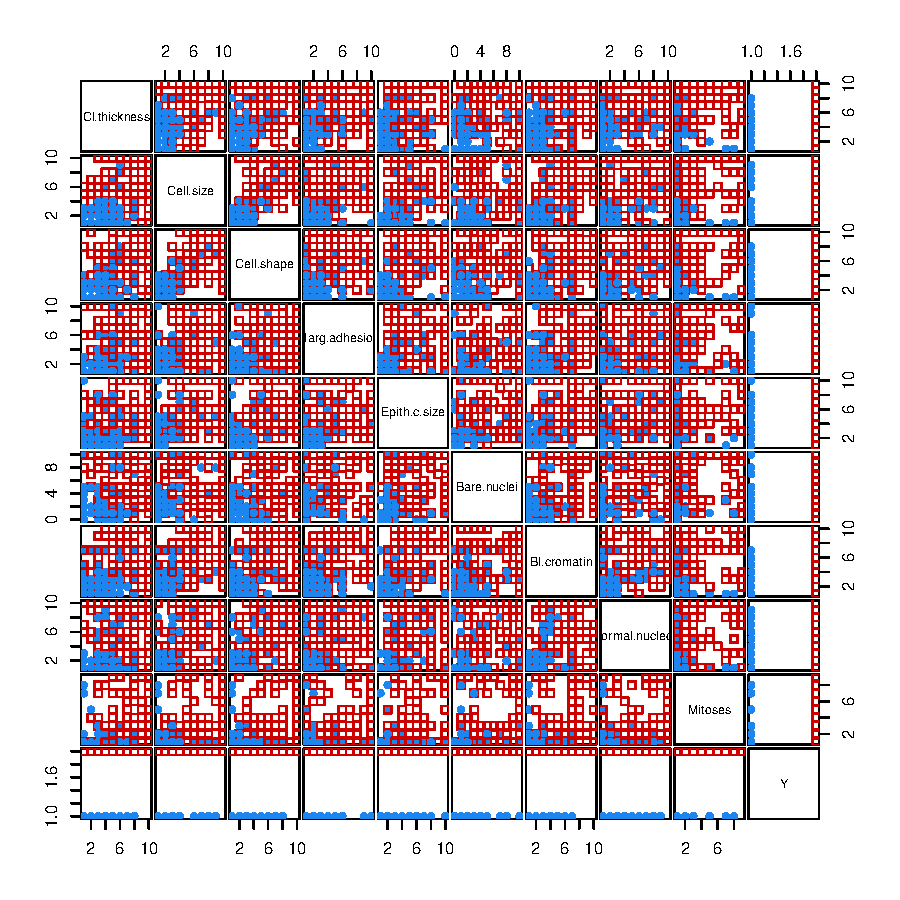
\includegraphics{selecao-002}

\begin{Schunk}
\begin{Sinput}
> ###########################
> # F-Score #
> f <- fscore(X,c1,c2,n)
> f
\end{Sinput}
\begin{Soutput}
[1] 1.1317247 1.8363064 1.8986351 0.8488204 0.8084139 1.8652137 1.3013896
[8] 0.9282550 0.1973198
\end{Soutput}
\end{Schunk}

\begin{Schunk}
\begin{Sinput}
> ###########################
> # Kmeans # 
> k <- list()
> for(i in 1:(nrow(t(X))-1))
+ {
+   h <- kmeans(t(X),i)
+   k[[i]] <- h$cluster
+ }
> k
\end{Sinput}
\begin{Soutput}
[[1]]
   Cl.thickness       Cell.size      Cell.shape   Marg.adhesion    Epith.c.size 
              1               1               1               1               1 
    Bare.nuclei     Bl.cromatin Normal.nucleoli         Mitoses 
              1               1               1               1 

[[2]]
   Cl.thickness       Cell.size      Cell.shape   Marg.adhesion    Epith.c.size 
              1               1               1               2               2 
    Bare.nuclei     Bl.cromatin Normal.nucleoli         Mitoses 
              1               1               2               2 

[[3]]
   Cl.thickness       Cell.size      Cell.shape   Marg.adhesion    Epith.c.size 
              3               2               2               2               2 
    Bare.nuclei     Bl.cromatin Normal.nucleoli         Mitoses 
              3               2               2               1 

[[4]]
   Cl.thickness       Cell.size      Cell.shape   Marg.adhesion    Epith.c.size 
              4               3               3               3               3 
    Bare.nuclei     Bl.cromatin Normal.nucleoli         Mitoses 
              3               3               1               2 

[[5]]
   Cl.thickness       Cell.size      Cell.shape   Marg.adhesion    Epith.c.size 
              3               3               3               2               3 
    Bare.nuclei     Bl.cromatin Normal.nucleoli         Mitoses 
              4               3               1               5 

[[6]]
   Cl.thickness       Cell.size      Cell.shape   Marg.adhesion    Epith.c.size 
              3               2               2               1               2 
    Bare.nuclei     Bl.cromatin Normal.nucleoli         Mitoses 
              4               2               6               5 

[[7]]
   Cl.thickness       Cell.size      Cell.shape   Marg.adhesion    Epith.c.size 
              6               2               2               7               4 
    Bare.nuclei     Bl.cromatin Normal.nucleoli         Mitoses 
              3               4               1               5 

[[8]]
   Cl.thickness       Cell.size      Cell.shape   Marg.adhesion    Epith.c.size 
              2               8               8               3               5 
    Bare.nuclei     Bl.cromatin Normal.nucleoli         Mitoses 
              4               6               7               1 
\end{Soutput}
\begin{Sinput}
> 
\end{Sinput}
\end{Schunk}
Analisando os resultados de clustering, pode-se ter uma noção da ordem de distinção espacial das características. Até 4 clusters, observamos que Cell.size, Cell.shape, Marg.adhesion, Epith.c.size, Bl.cromatin e Normal.nucleoli apresentam uma proximidade espacial significativa.
Ainda, observa-se que Mitoses, Cl.thickness e Bare.nuclei estão distantes dos demais grupos. Porém, Cl.thickness e Bare.nuclei distanciam-se de todas as outras características e apresentam alguma proximidade entre si, enquanto Mitoses está mais próxima do cluster citado anteriormente.

\begin{Schunk}
\begin{Sinput}
> ###########################
> # Hierarchical clustering #
> clusters <- hclust(dist(t(X)))
> plot(clusters)
\end{Sinput}
\end{Schunk}
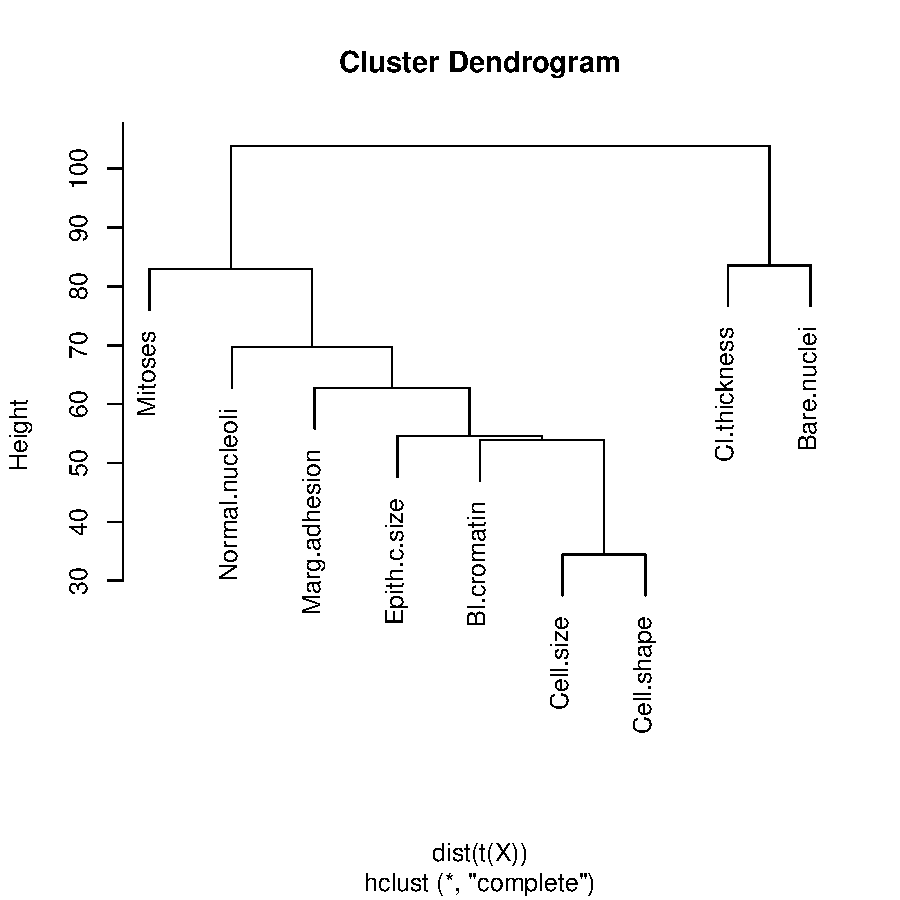
\includegraphics{selecao-005}

A partir dos resultados acima, pode-se observar a redundância dos atributos Cell.size e Cell.shape. Os resultados de clustering via kmeans demonstram uma proximidade espacial das duas características - agrupadas repetidamente no mesmo cluster. A distribuição comparativa dos atributos é elicitada no histograma a seguir:
\begin{Schunk}
\begin{Sinput}
> ###########################
> hist(t(X[,3]),col='red',xlab='Cell.size vs. Cell.shape',breaks=100,ylim=c(0,350))
> par(new=T)
> hist(t(X[,2]),col = 'blue', xlab='',breaks=100,ylim=c(0,350))
\end{Sinput}
\end{Schunk}
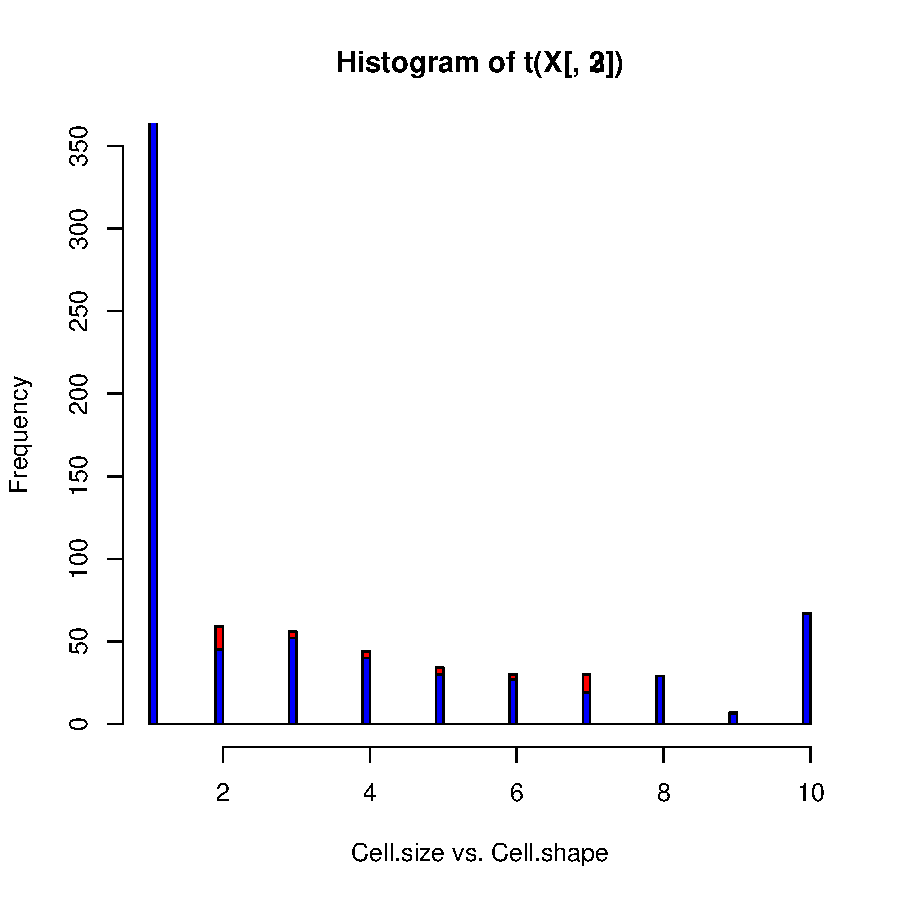
\includegraphics{selecao-006}
Caso seja necessária a redução de dimensionalidade do problema, é possível afirmar que a eliminação de uma das caractéristicas citadas acima não irá impactar na qualidade dos resultados. 
Comparando as características pertencentes ao mesmo cluster hierárquico, em ordem de similaridade:
\begin{Schunk}
\begin{Sinput}
> ###########################
> hist(t(X[,3]),col='red',xlab='Bl.cromatin vs. Cell.shape',breaks=100,ylim=c(0,350),xlim=c(0,10))
> par(new=T)
> hist(t(X[,7]),col = 'blue', xlab='',breaks=100,ylim=c(0,350),xlim=c(0,10))
\end{Sinput}
\end{Schunk}
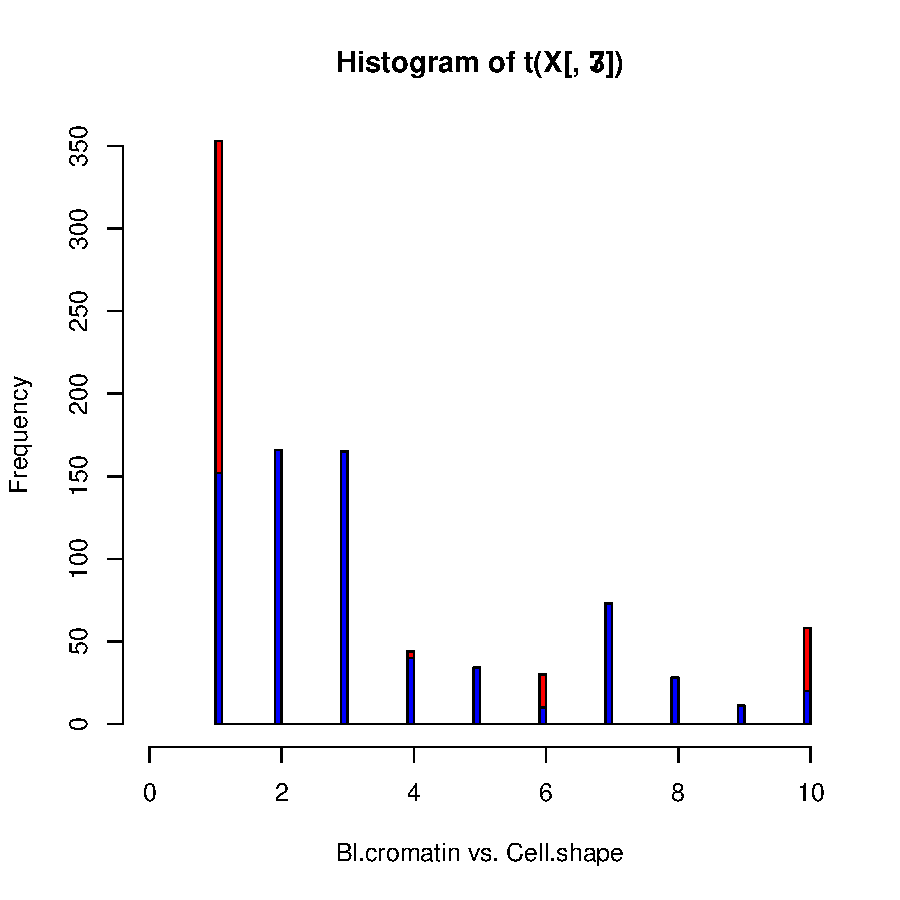
\includegraphics{selecao-007}

\begin{Schunk}
\begin{Sinput}
> ###########################
> hist(t(X[,5]),col='red',xlab='Bl.cromatin vs. Epith.s.size',breaks=100,ylim=c(0,350),xlim=c(0,10))
> par(new=T)
> hist(t(X[,7]),col = 'blue', xlab='',breaks=100,ylim=c(0,350),xlim=c(0,10))
\end{Sinput}
\end{Schunk}
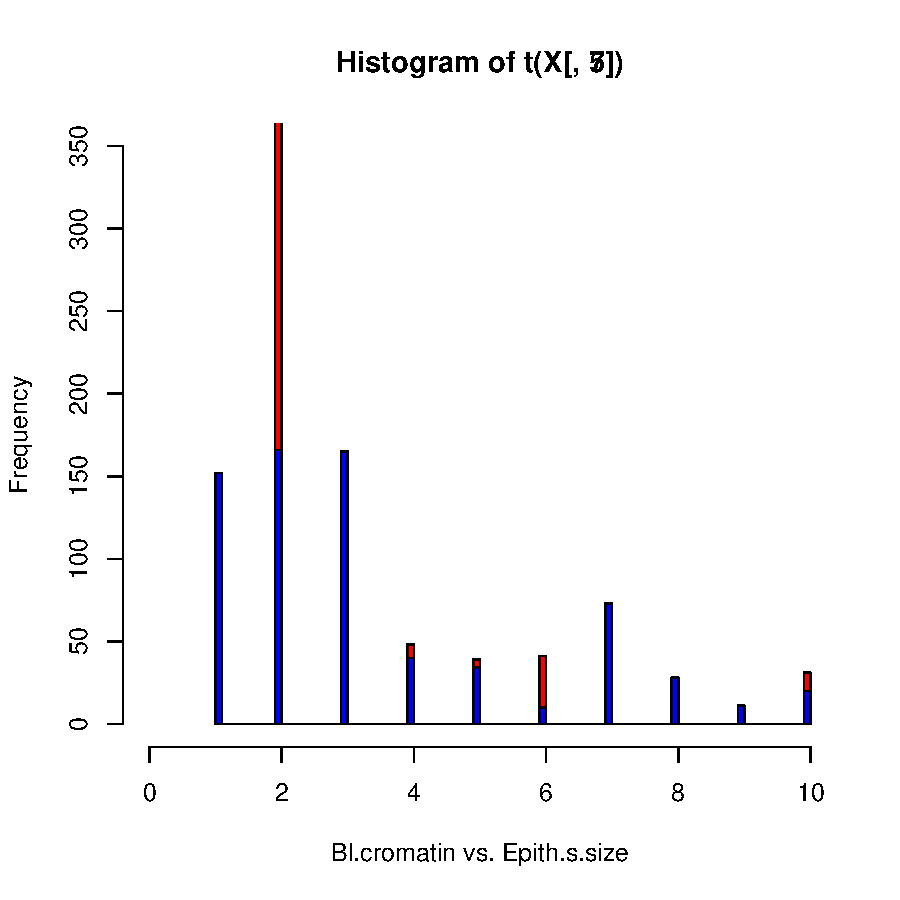
\includegraphics{selecao-008}

\begin{Schunk}
\begin{Sinput}
> ###########################
> hist(t(X[,4]),col='red',xlab='Bl.cromatin vs. Marg.adhesion',breaks=100,ylim=c(0,350),xlim=c(0,10))
> par(new=T)
> hist(t(X[,7]),col = 'blue', xlab='',breaks=100,ylim=c(0,350),xlim=c(0,10))
\end{Sinput}
\end{Schunk}
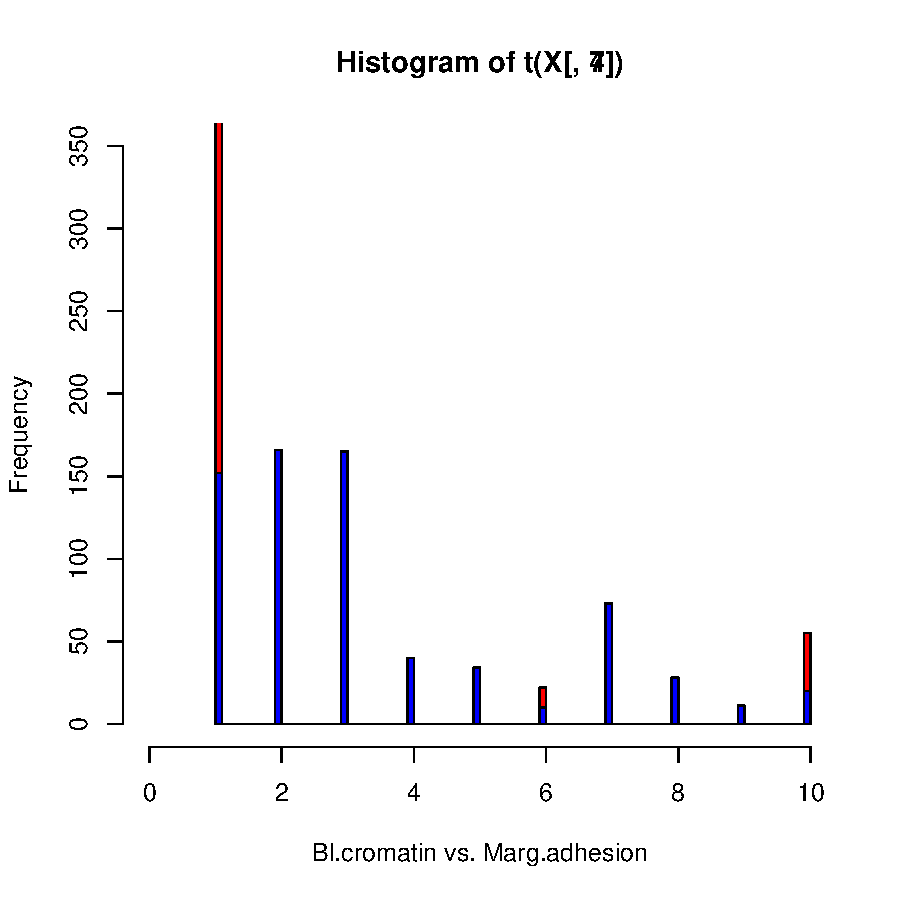
\includegraphics{selecao-009}

\begin{Schunk}
\begin{Sinput}
> ###########################
> hist(t(X[,4]),col='red',xlab='Bl.cromatin vs. Marg.adhesion',breaks=100,ylim=c(0,350),xlim=c(0,10))
> par(new=T)
> hist(t(X[,7]),col = 'blue', xlab='',breaks=100,ylim=c(0,350),xlim=c(0,10))
\end{Sinput}
\end{Schunk}
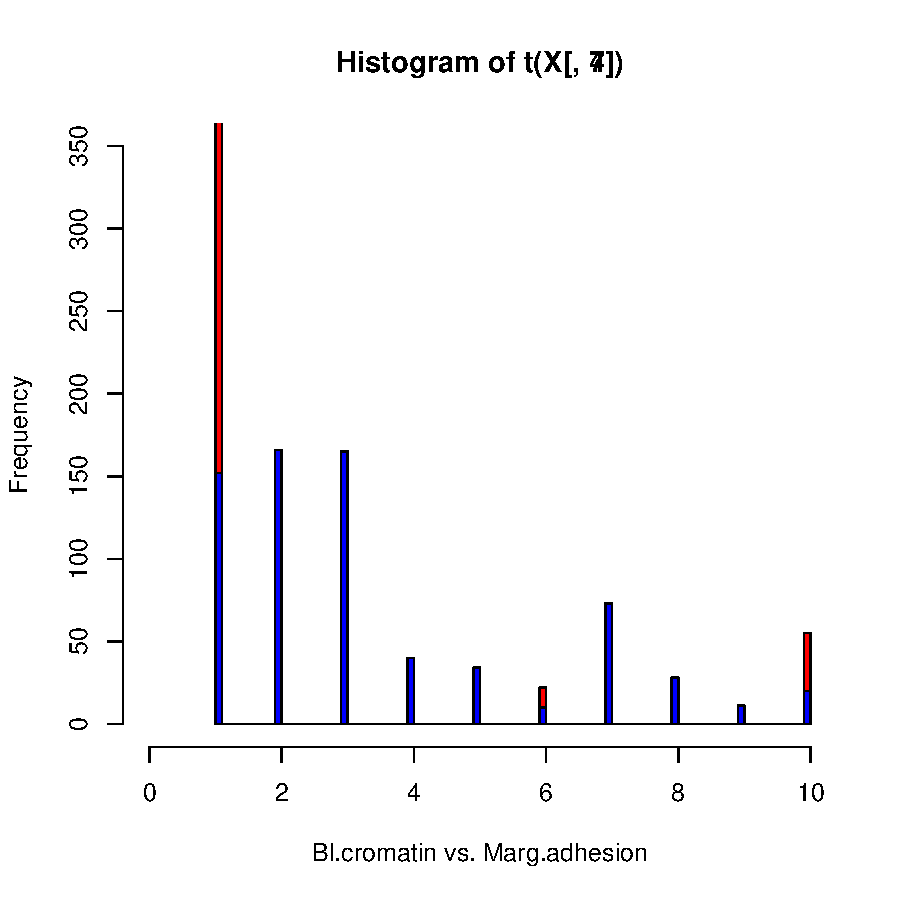
\includegraphics{selecao-010}

\begin{Schunk}
\begin{Sinput}
> ###########################
> hist(t(X[,8]),col='red',xlab='Bl.cromatin vs. Normal.nucleoli',breaks=100,ylim=c(0,350),xlim=c(0,10))
> par(new=T)
> hist(t(X[,7]),col = 'blue', xlab='',breaks=100,ylim=c(0,350),xlim=c(0,10))
\end{Sinput}
\end{Schunk}
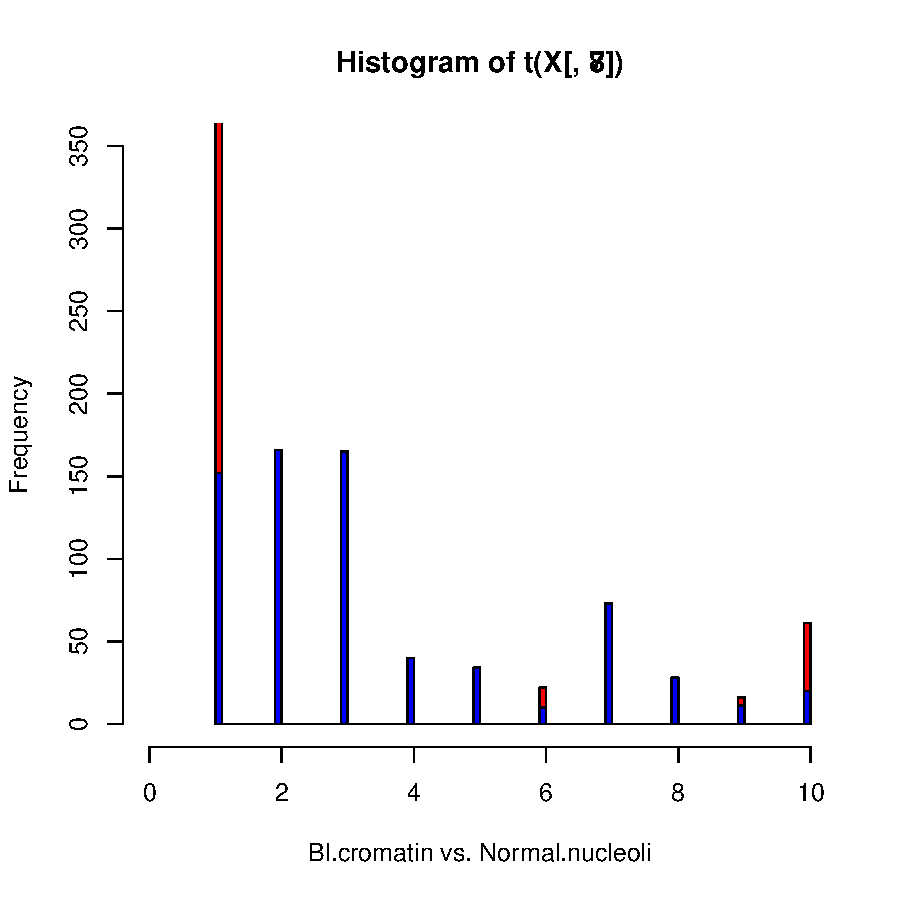
\includegraphics{selecao-011}

\begin{Schunk}
\begin{Sinput}
> ###########################
> hist(t(X[,9]),col='red',xlab='Bl.cromatin vs. Mitosis',breaks=100,ylim=c(0,350),xlim=c(0,10))
> par(new=T)
> hist(t(X[,7]),col = 'blue', xlab='',breaks=100,ylim=c(0,350),xlim=c(0,10))
\end{Sinput}
\end{Schunk}
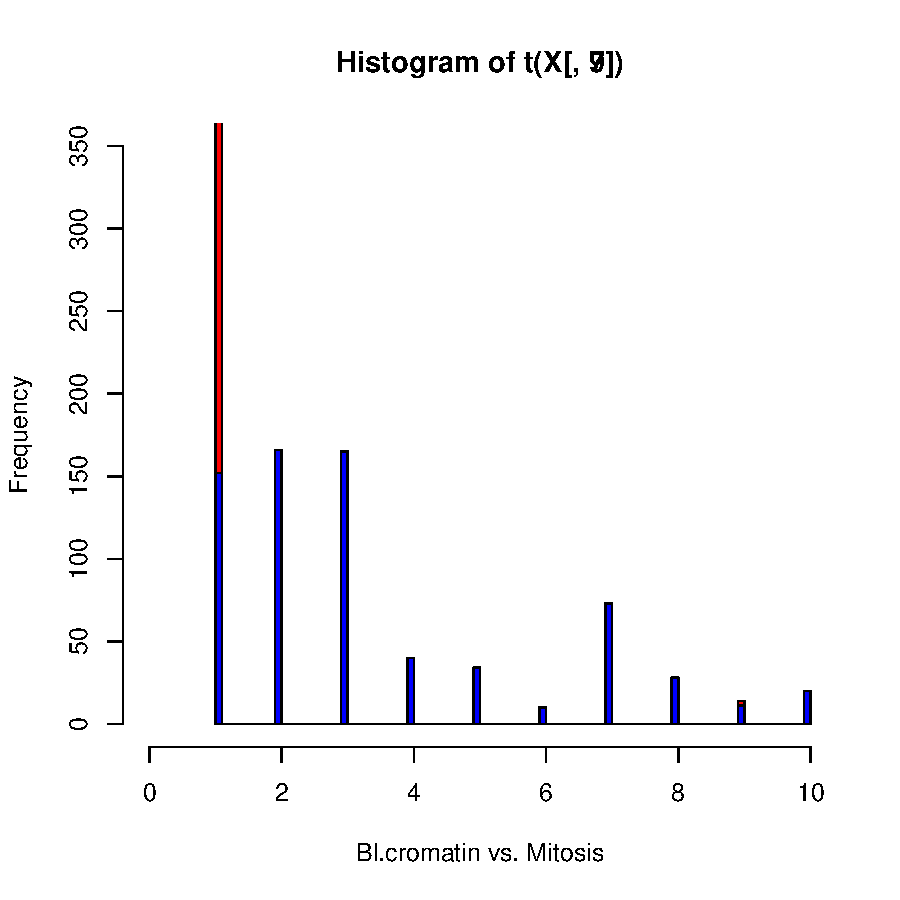
\includegraphics{selecao-012}

Comparando entre clusters:
\begin{Schunk}
\begin{Sinput}
> ###########################
> hist(t(X[,1]),col='red',xlab='Bl.cromatin vs. Cl.thickness',breaks=100,ylim=c(0,350),xlim=c(0,10))
> par(new=T)
> hist(t(X[,7]),col = 'blue', xlab='',breaks=100,ylim=c(0,350),xlim=c(0,10))
\end{Sinput}
\end{Schunk}
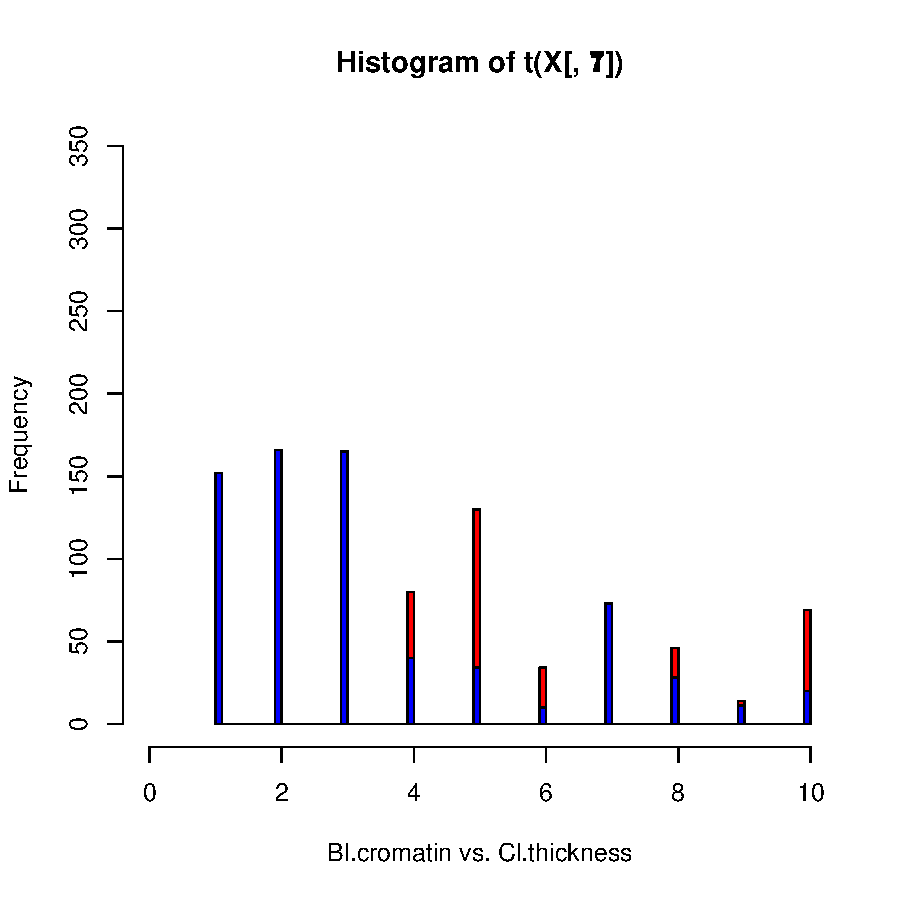
\includegraphics{selecao-013}

\begin{Schunk}
\begin{Sinput}
> ###########################
> hist(t(X[,6]),col='red',xlab='Bl.cromatin vs. Bare.nuclei',breaks=100,ylim=c(0,350),xlim=c(0,10))
> par(new=T)
> hist(t(X[,7]),col = 'blue', xlab='',breaks=100,ylim=c(0,350),xlim=c(0,10))
\end{Sinput}
\end{Schunk}
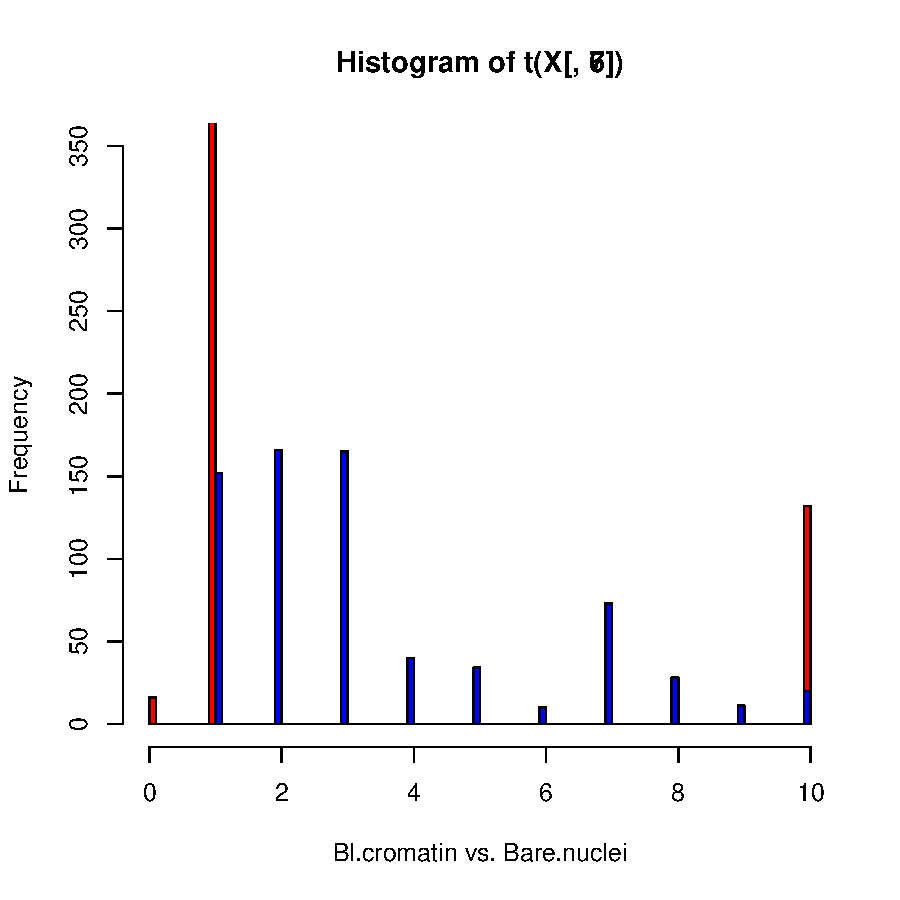
\includegraphics{selecao-014}
Observa-se que Cl.thickness apresenta uma distribuição mais próxima do cluster ao qual Bl.crompatin pertence, se comparada a Bare.nuclei.

\begin{Schunk}
\begin{Sinput}
> ###########################
> hist(t(X[,5]),col='red',xlab='Bare.nuclei vs. Mitosis',breaks=100,ylim=c(0,350),xlim=c(0,10))
> par(new=T)
> hist(t(X[,6]),col = 'blue', xlab='',breaks=100,ylim=c(0,350),xlim=c(0,10))
\end{Sinput}
\end{Schunk}
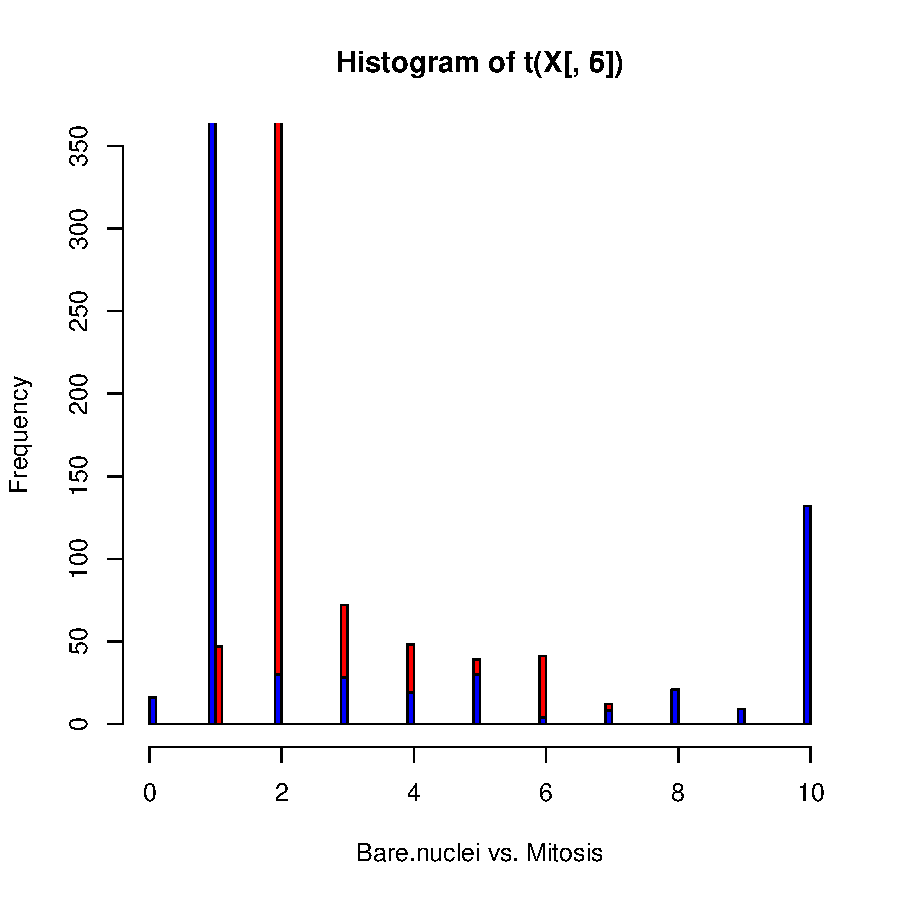
\includegraphics{selecao-015}

Comparação intra-cluster:
\begin{Schunk}
\begin{Sinput}
> ###########################
> hist(t(X[,1]),col='red',xlab='Bare.nuclei vs. Cl.thickness',breaks=100,ylim=c(0,350),xlim=c(0,10))
> par(new=T)
> hist(t(X[,6]),col = 'blue', xlab='',breaks=100,ylim=c(0,350),xlim=c(0,10))
\end{Sinput}
\end{Schunk}
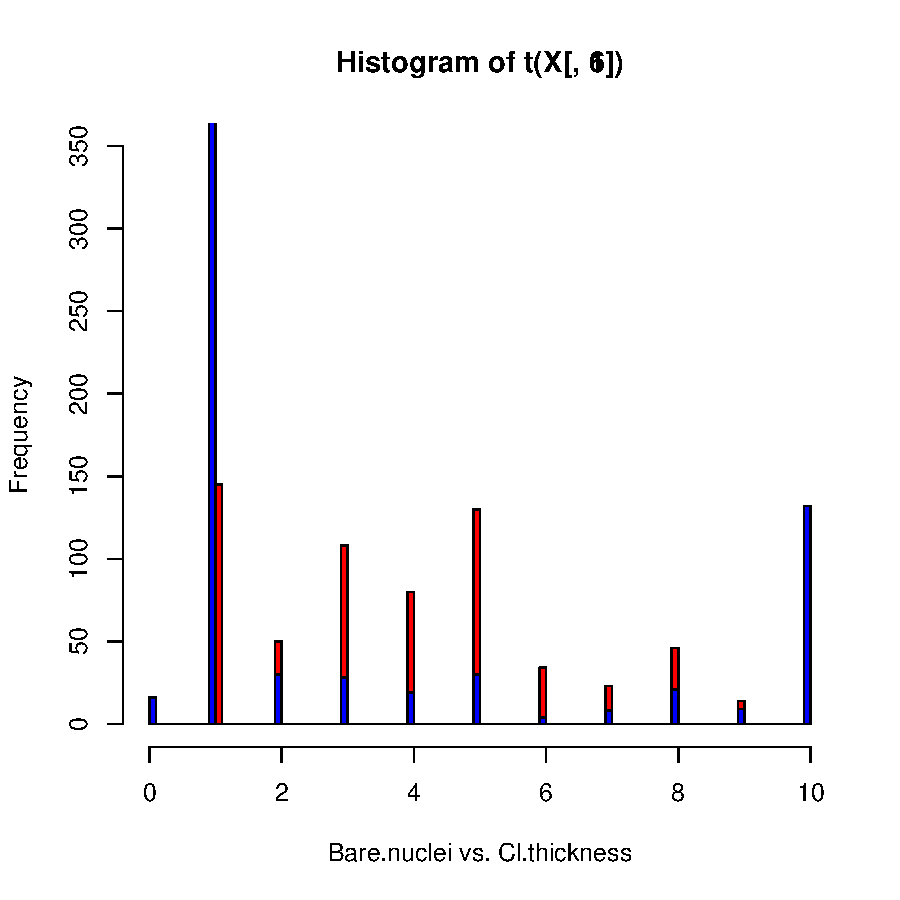
\includegraphics{selecao-016}

\end{document}
